\documentclass{article}
\usepackage[margin=1in]{geometry}
\usepackage{amsmath}
\usepackage{amsfonts}
\usepackage{amssymb}
\usepackage{bm}
\usepackage{graphicx}
\usepackage{caption}
\usepackage{subcaption}
\usepackage[bottom]{footmisc}
\usepackage{textcomp}
\usepackage{gensymb}
\usepackage[makeroom]{cancel}
\usepackage{pifont}
\usepackage{enumitem}
\usepackage{hyperref}
\usepackage[utf8]{inputenc}
\usepackage[english]{babel}
\usepackage{wrapfig}
\usepackage[framemethod=Tikz]{mdframed}

\usepackage{tikz,eepic}
\usepackage[mode=buildnew]{standalone}
\usetikzlibrary{patterns}

\renewcommand{\vec}[1]{\mathbf{\underline{#1}}}
\newcommand{\grad}{\nabla}
\newcommand{\cross}[2]{\vec{#1}\wedge\vec{#2}}
\newcommand{\crosso}[2]{\vec{#1}\wedge #2}
\numberwithin{equation}{section}
\newcommand*\dif{\mathop{}\!\mathrm{d}}
\newcommand*\Dif{\mathop{}\!\mathrm{D}}
\newcommand{\partder}[2]{\frac{\partial #1}{\partial #2}}
\newcommand{\partdero}[1]{\frac{\partial}{\partial #1}}
\newcommand{\fracder}[2]{\frac{\dif #1}{\dif #2}}
\newcommand{\fracdero}[1]{\frac{\dif}{\dif #1}}
\newcommand{\matder}[2]{\frac{\Dif #1}{\Dif #2}}
\newcommand{\matdero}[1]{\frac{\Dif}{\Dif #1}}
\newcommand*\ddif{\,\dif}


\newenvironment{rcases}
  {\left.\begin{aligned}}
  {\end{aligned}\right\rbrace}

\setlength{\footnotesep}{.3cm}
\setlength{\parskip}{1em}
\setlength{\parindent}{0em}

\newmdenv[backgroundcolor = black!10!white, roundcorner = 10pt, outerlinewidth=.5, leftmargin = 30, rightmargin = 30, innertopmargin =5pt]{aside}

\usepackage{biblatex}
\addbibresource{designdoc.bib}

% \usepackage[round,sort]{natbib}
% \bibliographystyle{abbrvnat}
\renewcommand{\floatpagefraction}{.8}


% \renewcommand{\bibname}{References}

\title{Finite Difference PDE Solver with Adaptable FD Scheme Implementation}
\author{Ari Gillman, Chemical and Biological Engineering,\\
James Roggeveen, Mechanical and Aerospace Engineering,\\
Kendra Bergstedt, Plasma Physics,\\
Ximing Li, Chemistry,\\
Princeton University
}
\date{January 2020}

\begin{document}
	\maketitle
	\section{Introduction}
		In this project we seek to design and develop software to solve PDEs using Finite Difference methods. In particular, we are interested in PDEs which may be solved by the method of strings. Our goal is to produce code that allows for particular finite difference schemes to be chosen by the user at runtime and to use these different discretizations to solve the PDE with no user manipulation of the governing equations. 
	\section{Background}
		PDE's are ubiqueteous in science and engineering, spanning everything from macroscopic energy and material transport to quantum mechanical descriptions of the unverse. Most of the PDEs encountered in scientific research may not be solved analytically and so numerical approximations are necessary to determine the solutions of these equations. Many such equations may be written in the form
		\begin{equation}
		\partder{\vec{u}}{t} = f\left(\vec{u},\partder{\vec{u}}{\vec{x}},\frac{\partial^2 \vec{u}}{\partial \vec{x}^2},\ldots \right)
		\end{equation}
		where $f$ is some function of the quantity of interest $\vec{u}$ and its spatial derivatives. Advection/diffusion equations, the heat equation, and the Navier-Stokes equations for example may all be written in this form. These equations may be numerically approximated by first evaluating $f$ using finite difference schemes to approximate the spatial coordinates. Then standard ODE solving schemes may be employed to solve the time problem. Finally, the boundary values are fixed subject to the boundary conditions. This is then repeated for the desired number of timesteps. 

		There are a large variety of finite difference schemes which may be employed to approximate the spatial derivatives. These schemes vary in terms of accuracy, stability, and computational cost. Our goal is to build software that is sufficiently modular that the user can specify the particular finite difference scheme at runtime. In addition, we want to allow the user relatively simple control over the process of implementing a new form of at PDE as well as adjusting the geometry of the given system. 

	\section{Architecture and Organization}
		The first main class to mention is the Problem class. This is where the approximate representation of the right-hand-side (spatial components only) of the PDE exists. The approximate representation is a combination of instances of the LinearOperator class, such as a derivative with respect to one spatial coordinate or a Laplacian operator. The Problem class also contains instances of the BoundaryCondition class that specify the boundary conditions for a given system. There is also an InitalCondition class that contains information about the system at the first time point, as well as a Grid class which contains information and methods pertaining to the geometry of the system. The Grid class also contains a GridFactory class that can be used to generate templates of the same size as the initial Grid instance. In order to generate the LinearOperators used in the Problem class, an OperatorFactory class is used in conjunction with a predefined finite difference scheme. To handle the boundary values after each time step, a BCHandler class is used.

		A SpatialDriver class calls the methods of the Problem and BCHandler classes in conjunction with the state variables at the current timestep to accomplish the first and third steps of the PDE algorithm. A TimeStepper class is used for the advancement of the state variables in time. This class simply implements a standard ODE integration scheme, such as Forward Euler or 4th Order Runge-Kutta. The Driver class orchestrates the calls to the SpatialDriver and TimeStepper classes in order to correctly execute the steps of the integration loop algorithm. The values of the state variables are written to a Logger class at the end of each loop and this data can be plotted or exported using a DataOutput class.

		To generate the appropriate LinearOperators which will be passed into problem, the code instantiates an instance of a Scheme subclass, which contains stencils for the basic linear derivatives discretized by that particular scheme. This Scheme subclass is then passed into the OperatorFactory, where it is used to generate a matrix representation of the discretized approximation to that linear operator. If the problem takes place on an $n\times m$ grid, the value of the function at each discretized point may be represented by a column vector of length $nm$. Then any linear opperator $\mathcal{L}$ may be approximated as
		\begin{equation}
			\mathcal{L}[\vec{u}] \approx A \cdot \vec{u}
		\end{equation}
		where $A$ is an $nm \times nm$ sparse matrix. Furthermore, linear vector operators may be constructed out of elementary derivative operators purely by linear transformations. Such operators improve the human readability of the equations expressed in the Problem class. These operator objects are all then passed into Problem upon its initialization. 

	\section{UML Diagram}
		(See Figure 1)
		\begin{figure}[h!]
			\centering
			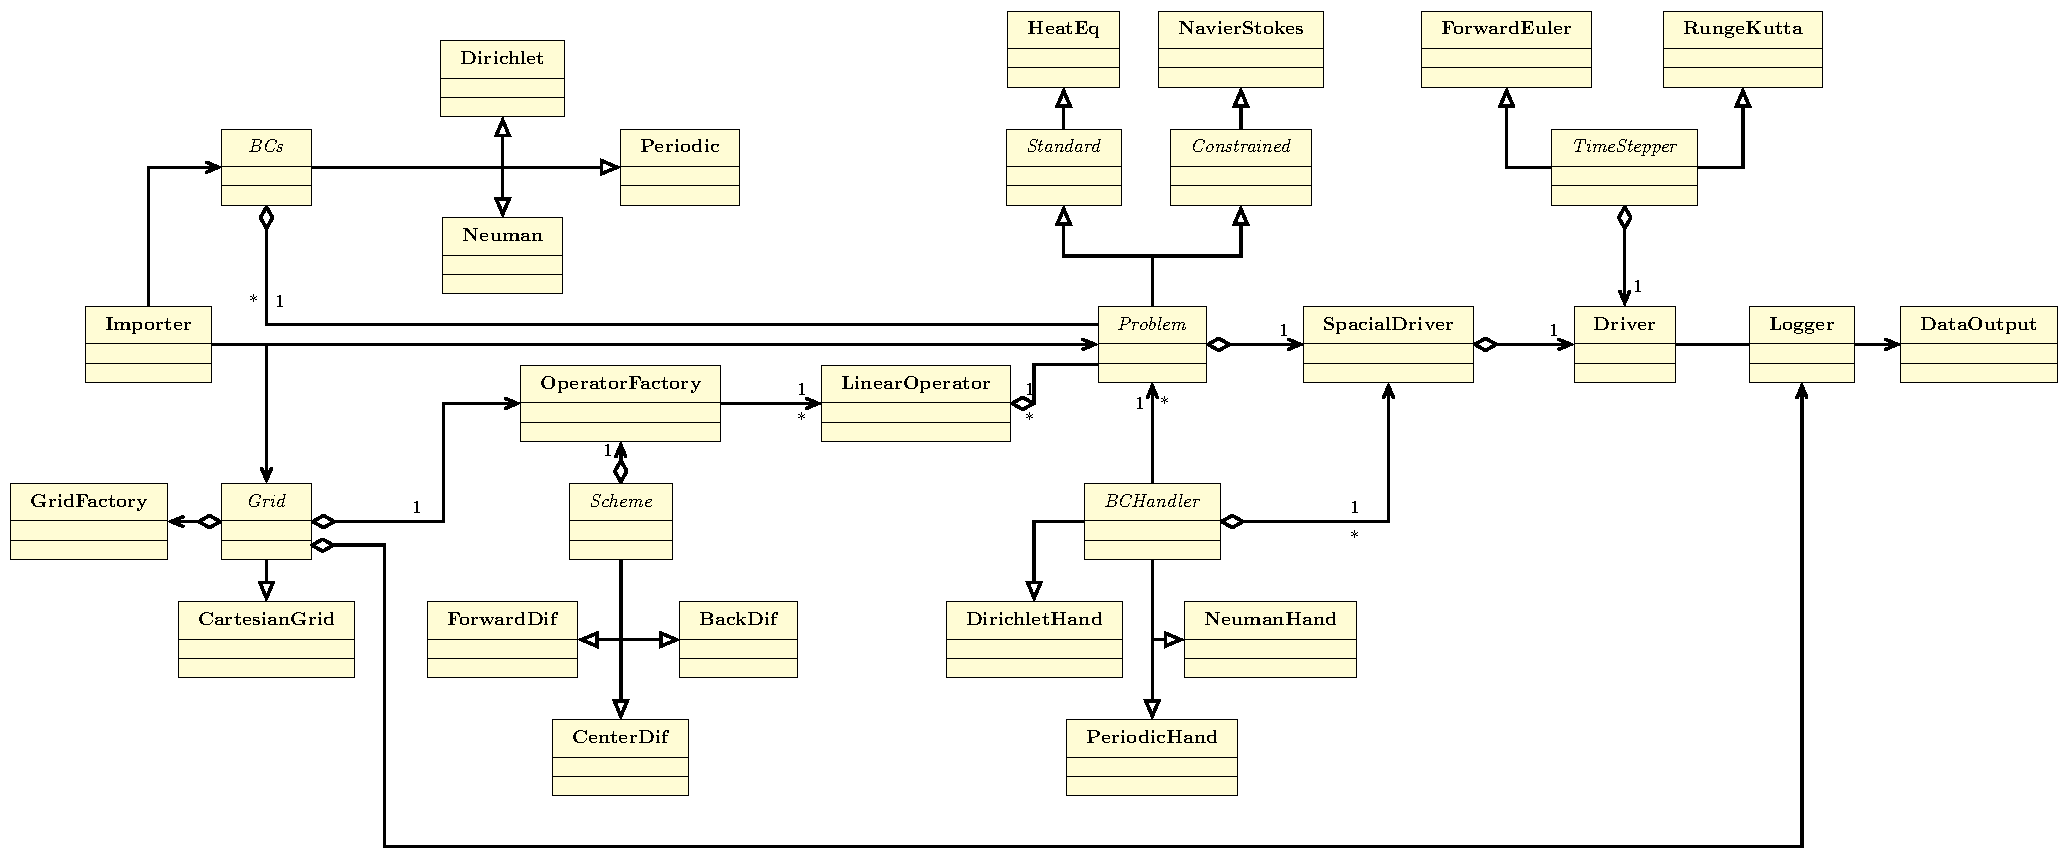
\includegraphics[angle=90,origin=c,width = .5\linewidth]{uml.pdf}
			\caption{Proposed UML diagram for our software.}
		\end{figure}	

	\section{Inputs}
		Prior to compilation the user must encode their specific PDE problem into a problem class, using the human-readable operators that the Operator Factor can produce. A long-term reach goal would be to turn this into something where the user can specify the equation at runtime and the Problem may be instantiated according to that input. 

		The user at runtime must supply the domain over which the equation is to be solved as well as the grid spacing. They must also specify the type and value of boundary condition at each edge (Dirichlet, Neumann, Periodic). They must supply their chosen discretization method for the RHS operators. The code should be sufficiently modular that the user could define a different discretization method for each implemented operator. 

		Additionally, the user supplies their desired time-domain stepper function as well as a timestep. The code checks the input timestep and grid step to ensure it meets the criteria for stability. The user may also be able to choose desired output methods. 

	\section{Computation}
		The finite difference approximations to linear operators will be represented as large, sparce matricies, where the non-zero elements correspond to the appropriate linear combination of neighboring function values. The inner product of these matricies with a vector of discretized function values returns a vector of values corresponding to the application of the operation to the function. These vectors may then be combined to determine the right hand side of the PDE. Note that while the operators are linear they may be combined in a non-linear fashion by the Problem.

		As an examble the first order center difference approximation for a discretized function $u$ is given by $\frac{1}{2h^2}f_{i+1} - 2 f_{i} + f_{i-1}$ where $h$ is the spatial discretization parameter and $i$ the index of the spatial coordinate. This would in turn correspond to a matrix of the form
		\begin{equation}
		\frac{1}{2 h^2} \left(
		\begin{matrix}
		1 & -2 & 1 & 0 & 0 \\
		0 & 1 & -2 & 1 & 0 \\
		0 & 0 & 1 & -2 & 1
		\end{matrix}\right)
		\end{equation}
		for a particular subsection of the operator matrix. As part of the OperatorFactory the operator matrix will also be updated to apply different schemes to the edge values of the operator if the normal stencil would overrun. 

		All of the computation to generate the operators is overhead at runtime. Once they have been created and passed to problem, calculation of the RHS of the equation is limited only by the speed at which the linear algebra operations may be performed.

		After the RHS of the equation are evaluted the equation may be advanced in time using a simple ODE time solver, such as Forward Euler. 

	\section{Validations}
		We will be validating our code by 
		\begin{itemize}
			\item Verifying the correctness of the linear operators by approximating derivatives of known functions
			\item Comparison of results for 1D and 2D heat equation models with dirichlet boundary conditions for various initial conditions
		\end{itemize}


	\nocite{pycfd}
	\nocite{*}
	% \bibliography{designdoc}
	\printbibliography

\end{document}
